\documentclass[conference]{IEEEtran}
\IEEEoverridecommandlockouts
% The preceding line is only needed to identify funding in the first footnote. If that is unneeded, please comment it out.
\usepackage{cite}
\usepackage{amsmath,amssymb,amsfonts}
\usepackage{algorithmic}
\usepackage{graphicx}
\usepackage{caption}
%\usepackage{subfigure}
\usepackage{subcaption}

\usepackage{textcomp}
\usepackage{listings}
\usepackage{multicol}
\usepackage{tikz}

\newcommand{\fixme}[1]{{\color{red}\textbf{FIXME:} #1}}
\newcommand{\Ehsan}[1]{{\color{blue}\textbf{Ehsan:} #1}}
\newcommand{\Fatem}[1]{{\color{green}\textbf{Fatemeh:} #1}}
\newcommand{\Marjan}[1]{{\color{cyan}\textbf{Marjan:} #1}}

\usepackage{xcolor}
\def\BibTeX{{\rm B\kern-.05em{\sc i\kern-.025em b}\kern-.08em
		T\kern-.1667em\lower.7ex\hbox{E}\kern-.125emX}}
\newcommand{\conn}{\!\rightsquigarrow\!}
\newcommand{\nconn}{\!\mathrel{\hspace{.1em}\not\hspace{-.1em}\rightsquigarrow}\!}
\newcommand{\overto}[1]{\stackrel{#1}{%
		\overrightarrow{\smash{\,{\phantom{#1}}\,}}}}

%-------------------------
\lstdefinelanguage{rebeca}{
	morekeywords={reactiveclass, knownrebecs, statevars, main, msgsrv, constraints,con, main, define, LTL, CTL, boolean, int, shortint, byte, if, else, while, for, wait, msg, reset, set, self, false, true, now, after, delay, deadline, initial, unicast, succ, unsucc},
	otherkeywords={=>,<-,<\%,<:,>:,\#,@},
	sensitive=true,
	morecomment=[l]{//},
	morecomment=[n]{/*}{*/},
	morestring=[b]",
	morestring=[b]',
	morestring=[b]"""
}
%\captionsetup[lstlisting]{font={small}}
\lstset{
	language=rebeca,
	aboveskip=3mm,
	belowskip=3mm,
	showstringspaces=false,
	columns=flexible,
	xleftmargin=10mm,
	% basicstyle={\myttsize\ttfamily},
	basicstyle={\small},
	keywordstyle=\color{blue},
	numbers=left,
	numberstyle=\color{black},
	numbersep=7pt,
	stepnumber=1,
	breaklines=true,
	breakatwhitespace=true,
	tabsize=2,
	numberblanklines=false,
	frame=l
}

\begin{document}
	
	\title{%Reactive Actors in Isolation for Efficient Analysis \\
	Reactive Actors: Isolation for Efficient Analysis 
		\thanks{The authors would like to acknowledge DPAC and SEADA.}
	}
	
	\author{\IEEEauthorblockN{Marjan Sirjani}
\IEEEauthorblockA{
\textit{School of Innovation, Design and Engineering} \\
\textit{M{\"a}lardalen University}\\
V{\"a}ster{\aa}s, Sweden \\
\textit{School of Computer Science} \\
\textit{Reykjavik University}\\
Reykjavik, Iceland \\
marjan.sirjani@mdh.se}
		\and
		\IEEEauthorblockN{Ehsan Khamespanah}
\IEEEauthorblockA{\textit{School of Computer Science} \\
\textit{Reykjavik University}\\
Reykjavik, Iceland \\
\textit{ School of ECE} \\
			\textit{University of Tehran}\\
			Tehran, Iran \\
ehsank@ru.is}
		\and
		\IEEEauthorblockN{Fatemeh Ghassemi}
		\IEEEauthorblockA{\textit{ School of ECE} \\
			\textit{University of Tehran}\\
			Tehran, Iran \\
			fghassemi@ut.ac.ir}
	}
	
	\maketitle
	
	\begin{abstract}
		In this paper, we will introduce timed reactive actors for modeling distributed systems and will explain our theories, techniques and tools for model checking and performance evaluation of such models.  Rebeca can be used to model asynchronous event-based components in systems, and in the extended version, Timed Rebeca, real time constraints can be captured in the language. We will explain how the isolation of actors, meaning no shared variable, non-preemptive execution of event handlers, and no blocking send or receive, help in developing more efficient analysis techniques. We show how floating-time transition system can be used for model checking of such models when we are interested in event-based properties, and how it helps in state space reduction. We explain how isolation of actors helps in distributed model checking? ... and how it helps in verification of MANETs. The same approach can be used in verification of swarms ...
		
		%I will show different applications of our approach including analysing a wireless sensor network application, mobile ad-hoc network protocols, network-on-chip designs, and a macroscopic agent-based simulation of urban planning.
	\end{abstract}
	
	\begin{IEEEkeywords}
		Actors, Real-time systems\end{IEEEkeywords}
	
\section{Introcution} \label{sec::introduction}

%\Marjan{Add your comments in others' sections in color}\Ehsan{blue}\Fatem{green}

%Message of the paper: The actor-based language, Rebeca, provides a usable and analyzable model for distributed, concurrent, event-based asynchronous systems (Cyber-Physical systems).

%Distributed systems  are defined like this
%IBM: A distributed computer system consists of multiple software components that are on multiple computers, but run as a single system. The computers that are in a distributed system can be physically close together and connected by a local network, or they can be geographically distant and connected by a wide area network. ...distributed system contains multiple nodes that are physically separate but linked together using the network. All the nodes in this system communicate with each other and handle processes in tandem. Each of these nodes contains a small part of the distributed operating system software.

Distributed systems consist of software components executed on different computers that are linked together by a network. The software components communicate with each other in order to achieve the goal of the distributed system.
Nowadays distributed systems are everywhere providing scalability and redundancy.  Design and analysis of such systems is overly challenging.

%Reactive systems are defined like this
%Actor-based languages and distributed systems
Actor model is a model of concurrent computation for developing parallel, distributed and mobile systems \cite{Hewitt:77:Actors,Agha:97:ActorComputation}. Each actor is an autonomous object that operates concurrently, and  send and receive messages asynchronously.
%
Rebeca \cite{DBLP:journals/fuin/SirjaniMSB04,DBLP:conf/fmco/Sirjani06} is an actor-based language proposed to bridge the gap between software engineers and formal methods community.
Rebeca comes with a formal semantics and is the first actor-based language with model checking support \cite{DBLP:journals/csur/BoerSHHRDJSKFY17}.


Models can be used for both synthesis and analysis \cite{DBLP:conf/facs2/LeeS18}. We build abstract models that serve as a specification of a system to be built, and then we refine the models, adding
details until we build the system itself. The process is usually iterative, with
the specifications evolving along with their refinements. We may have different analysis purposes like verification, validation, and performance evaluation. 
Model checking, simulation, and building physical prototypes can all be used as methods for analysis. Simulation, which is the execution of an executable
model, reveals one possible behavior of a model with one set of inputs. Model
checking reveals all possible behaviors of a model over a family of inputs \cite{DBLP:conf/facs2/LeeS18}.
%If we have formal and automatic refinement techniques, we may be able to avoid introducing errors in the refined models while details are added. In this case, synthesis is said to be “correct by construction.”


%Why actors are good models for distributed systems?
%\noindent\textbf{Faithful models for distributed reactive systems} %\label{sec::Faithfulness}
%How models shape the thought and ease the analysis

%From Rocco paper: 
According to De Nicola et.al. in \cite{DBLP:conf/coordination/NicolaFPT18} a major challenge in designing languages is to devise appropriate abstractions and linguistic primitives to deal with the specificities of the domain under investigation.
%
%From Gul and Rajesh: 
%http://web.cs.ucla.edu/~palsberg/course/cs239/papers/karmani-agha.pdfA 
Karmani and Agha believe that a programming language should facilitate the process of writing programs by being close to the conceptual level at which a programmer thinks about a problem, rather than at the level at which it may be implemented \cite{DBLP:reference/parallel/KarmaniA11}.
%
In \cite{DBLP:conf/birthday/FriendlinessSirjani18}, Sirjani defines faithfulness as the similarity of the
model and the system; and it is argued that faithfulness can bring in analizability and tracability. 
According to \cite{DBLP:conf/birthday/FriendlinessSirjani18}, a modeling
language is faithful to a system if the model of computation supported by the
language matches the model of computation of [the features of interest of] the
system. 
In \cite{Ptolemy:14:Book} a model of computation (MoC) is defined as a collection of rules that govern
the execution of the [concurrent] components and the communication between
components.
Faithfulness can be seen as the key motivation behind domain-specific
languages.

%\Marjan{Here I should add: Rebeca is designed to be faithful to ... At the same time we considered analyzability and so keeping things as simple as possible.Theories and tools are developed (cite papers). Rebeca is used in different applications (cite papers), and each application we devised new techniques mostly using the adavntage of isolation.}

Rebeca is designed as a \textit{faithful} language for distributed software systems.
It is an imperative actor-based language while original actor languages are mainly functional languages. It is an event-driven and asynchronous language, with implicit receive and non-blocking send statement. There is no shared variables, and methods are atomic and run to completion.
A  tool suite for model checking is available at \cite{RebecaSite}. Theories, techniques and tools for compositional verification \cite{DBLP:journals/jucs/SirjaniMSB05}, symmetry and partial order reduction \cite{DBLP:journals/acta/JaghooriSMKM10}, and slicing \cite{DBLP:journals/scp/SabouriS10}  are proposed. All the above methods are based on techniques using isolation of actors.
Rebeca is used for schedulability analysis of wireless sensor network applications \cite{DBLP:journals/sttt/KhamespanahSMA18}, protocol verification\cite{FOAC}, design exploration  and comparing routing algorithms \cite{DBLP:journals/eceasst/sharifiMMS13}. It is also used for lightweight preprocessing for agent-based simulation \cite{DBLP:journals/scp/BerardinisFJS18}. 


In the following section we explain what we mean by isolation of actors and how it can help in analysis. We then focus on a model that is presented as the semantics of Timed Rebeca and can help by a significant amount of reduction in the state space while doing the analysis. We believe that similar techniques can be used in different analysis methods for event-based reactive isolated modules. 
%
In Section \ref{sec::DMC}, we present a technique used for analysis by distributed model checking which is specific for actors. The efficiency of the technique is checked for model checking Rebeca models.
%
Section \ref{sec::wrebeca} explains how we deployed special techniques to make analysis of  mobile adhoc networks possible.

%\noindent\textbf{Analysis of distributed systems and isolated actors.}
\section{Analysis of Distributed Systems and Isolated Actors}
For explaining our approach, we distinguish three levels of abstraction: the distributed software system itself with all the implementation details, the modeling language which is Rebeca here, and the generated state space which is built for the sake of analysis and  we model it as a state transition system. There are alternative ways for analysis, like using logical theorems and applying reasoning based on that, but here we use different variations of state transition systems.
We sometimes call the transition system the semantics of our model as it shows the behavior in a formal way.


Active objects and actors are encapsulated modules with no shared variables. In Rebeca, we also choose to have atomic execution of message servers (i.e. methods, or event handlers) which gives us a macro-step semantics and models a non-preemptive execution of the handlers.
\Marjan{I should add here that why we can have atomic method execution without loss of generality, and ... maybe how we can model preemption?}
Our actors are reactive, when sending a message they are not blocked and there is no explicit receive. So, there is no coupling via shared variables, no coupling because of waiting for another actor to return a value for a remote procedure call, and no coupling because of a context dependency caused by having a \textit{future}  construct in the language.
This isolation of actors helps in more efficient analysis, and reduces the state space.
Moreover, if we are only interested in the event-based properties we may be able to abstract even more and just keep the states that are followed by a transition which we are interested in. This type of reduction is not straight forward as we need to prove that we are preserving the order of the events while abstracting away some of the states and transitions. 
%This is what is done in partial order reduction.

Floating Time Transition System is a natural event-based semantics for timed actors, giving us a significant amount of reduction in the state space, using a non-trivial novel idea.
	
%paragraphs in the Intro
%%\section{Reactive Systems} \label{sec::reactive-systems}
\paragraph{Reactive Systems} \label{sec::reactive-systems}
%\section{Reactive Actors} \label{sec::reactive-actors}

%\paragraph{Faithful Models for Reactive Systems} \label{sec::Faithfulness}
From Rocco paper: a major challenge in designing languages is to devise appropriate abstractions and linguistic primitives to deal with the specificities of the domain under investigation.

\section{Timed Rebeca and Floating Time Transition System} \label{sec::FTTS}

Timed Rebeca is an extension of Rebeca where we can model computational time, network delays, and periodic events \cite{Arni}.

Floating Time Transition System (FTTS) is proposed based on the isolation of timed rebecs \cite{FACS2015,SCP}. The idea behind FTTS is similar to partial order reduction (POR) but the technique does not fit exactly in the definition of POR. What we mean by floating time is that in each state of the state space, different actors do not necessarily have the same local clock, i.e.,  actors are not synchronised on their local time in the state space. We consider this as letting the time \textit{float} across the actors in the state space. 
To avoid confusion, it is important to note the different models in different levels of abstraction, and also layering of models. We have (1) distributed systems, we use (2) Timed Rebeca to model distributed systems, and we model (3) the state space as Floating Time Transition System to do the analysis. 
%
Note that at the level of Timed Rebeca, actors have synchronised local clocks which gives us a notion of global time across the model. We use time stamps, and time stamps are comparable across all actors in the model. This makes our model simpler and more understandable, and our analysis more efficient.
But in distributed systems we cannot assume synchronised clocks and time stamps. 
For that assumption to be valid and faithful enough to the system,  we rely on the layering and different responsibilities for different layers. For distributed actors (as faithful representatives of distributed software components) to be able to have synchronised clocks and comparable time stamps we rely on the lower-level network protocols to provide that for us. 

In Timed Rebeca we have a concept of time and we can consider that each statement is executed at a certain point in time. Note that we are now talking at the level of the Rebeca model, the notion of time is the model time, and we do not need to worry about synchronising the clocks among different components in the distributed system. We assume that local clocks of actors are synchronised and we can have comparable time stamps on each statement in the actors.
%
In Timed Rebeca models, we use a \texttt{delay(t)} statement to show the computation delay. Other statements are assumed to be executed in zero time. We use  \texttt{after(t)} in combination with a \texttt{send} message statement, it means that the time stamp of the message when it is put in the queue of the receiver is the value of the local clock of the sender (\texttt{now} in the sender) plus the value of \texttt{t}.
The progress of time is forced by the \texttt{delay} statement and also by \texttt{after}. 
We can assume that the time stamp of all the statements are zero when a model starts to execute, then in each actor the local time is increased by value of \texttt{t} if there is a \texttt{delay(t)} statement.
A \texttt{send} statement with an  \texttt{after} does not cause any increase in the local time per se. The statement following the \texttt{send} statement has the same time stamp as the \texttt{send} statement itself.
The \texttt{after} construct may cause an increase in the time when the actor picks the message annotated by \texttt{after} to be executed. The local time of the receiver actor is set to the time stamp of the message, unless it is already greater than that.
The latter situation means that the message has been sitting in the queue while the actor has been busy executing another message.
Remember that messages are executed atomically and are not preempted.
%
The progress of time happens in the case that the time stamp of the message is greater than the local time of the receiver actor, the local time will be pushed forward.
%
The \texttt{after} construct can be used to model the network delay, and also to model periodic events.


If we use the standard Timed Transition System (TTS) to generate the state space for Timed Rebeca model we distinguish three types of transitions: $\tau$ transitions, \textit{events}, and \textit{timed} transitions.
In FTTS we reduce that to only \textit{events} transitions.
%
We explain TTS and FTTS for Timed Rebeca using an example in Listing \ref{src::FTTS-actor-model}.
Listing \ref{src::FTTS-actor-model} shows a simple Rebeca model with two rebecs $r1$ and $r2$ instantiated from two reactive classes $RC1$ and $RC2$.
$RC1$ has only one message server ($m1$) in which it triggers the two message servers of $RC2$ ($m2$ and $m3$).
The two message servers of $RC2$ are event handlers that do nothing, i.e., there are no internal actions caused by statements like assignments, or \texttt{send}, and no  \texttt{delay} statements. Note that \texttt{send} statements are considered as internal or silent actions but they cause a change in the message queue of the receiver by adding the sent message to that queue.
 

Figure \ref{fig::FTTSandTTS}.a shows the TTS generated for the model in Listing \ref{src::FTTS-actor-model}. 
The constructor of $RC1$ puts the message $m1$ in the queue of $RC1$. So, in $time=0$ we have the message $m1$ in the queue of $r1$ (see state $s_0$ in Figure \ref{fig::FTTSandTTS}.a). Also, you see that the message queue of $r2$ is empty. On the transition from $s_0$ to $s–1$ the message is taken from the queue of $r–1$, and in the state $s_1$ the method $m_1$ is ready to be executed, i.e., the Program Counter (PC) is at $m1:1$. The first statement in $m_1$ is a \texttt{delay} statement which is executed and pushes the time forward to $time=2$ in state $s_2$.
In the state $s_2$, the PC points at a $send$ statement: $r_2.m_2()$. After this statement is executed as a silent or $\tau$ statement, we have the message $(r_1 \rightarrow r_2.m_2(), 0, \infty)$ in the queue of $r–2$


\begin{lstlisting}[language=rebeca, caption= A simple Timed Rebeca model with two rebecs, label=src::FTTS-actor-model]
reactiveclass RC1 (3) {
	knownrebecs {
		RC2 r2;
	}
	RC1() {
		self.m1();
	}
	msgsrv m1() {
		delay(2); %PC = 1
		r2.m2();  %PC = 2 
		delay(2); %PC = 3 
		r2.m3();  %PC = 4
		self.m1() after (10); %PC = 5
	}
}
reactiveclass RC2 (4) {
	knownrebecs {
		RC1 r1;
	}
	RC2() { }
	msgsrv m2() { }
	
	msgsrv m3() { }
}

main {
	RC1 r1(r2):();
	RC2 r2(r1):();
}

\end{lstlisting}

\begin{figure}
\centering
\begin{subfigure}[b]{0.2\textwidth}
%\subfigure[TTS]{
%\label{fig::TTS}
  \centering
  \small{
   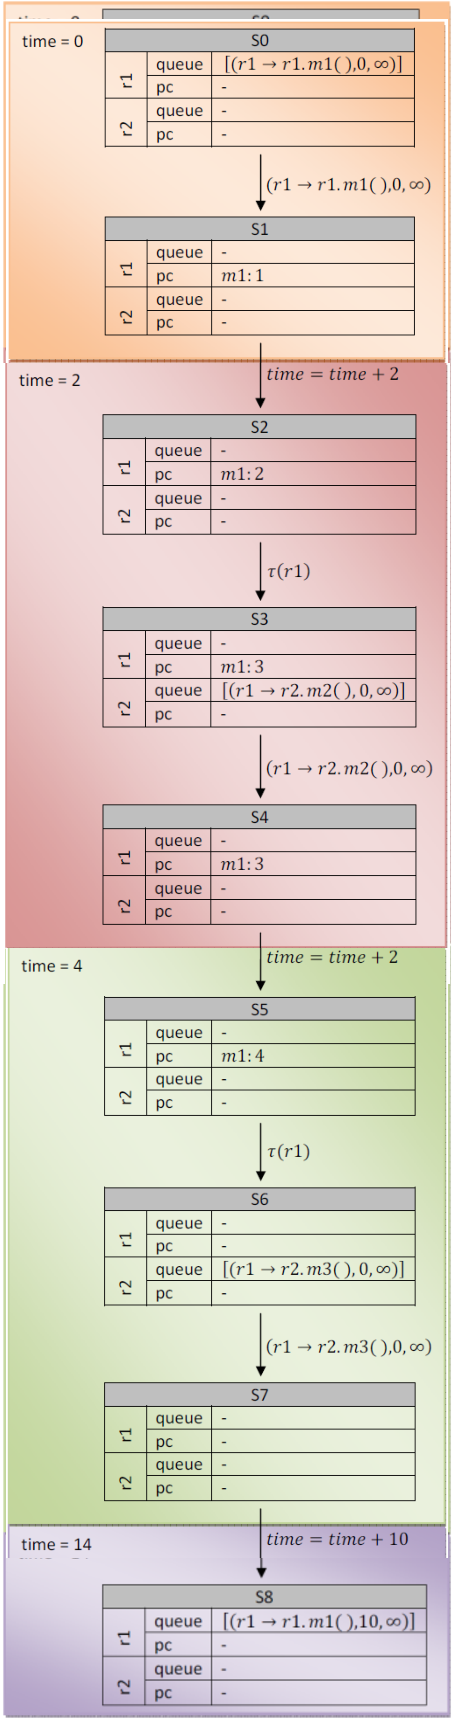
\includegraphics[width=.8\textwidth]{TTSCorrect.pdf}
  }
  \caption{TTS}
  \label{fig::TTS}
%}
\end{subfigure}
%\qquad
\begin{subfigure}[b]{0.2\textwidth}
%\subfigure[FTTS]{
%\label{fig::FTTS}
  \centering
  \small{
   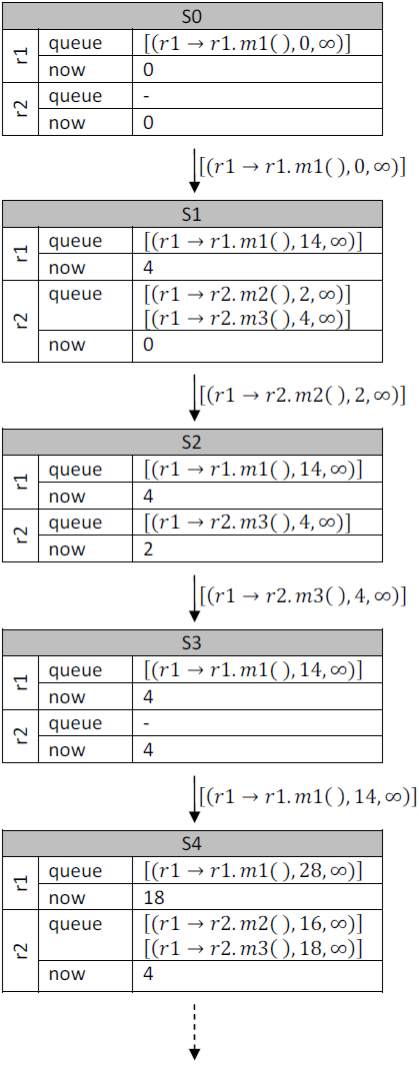
\includegraphics[width=.8\textwidth]{Picture2-FTTS.pdf}
   \caption{FTTS}
   \label{fig::FTTS}
  }
%}
\end{subfigure}
\caption{ TTS and FTTS for the Timed Rebeca model in Listing \ref{src::FTTS-actor-model}.}
\label{fig::clinger-cdg}
\end{figure}

\begin{figure}
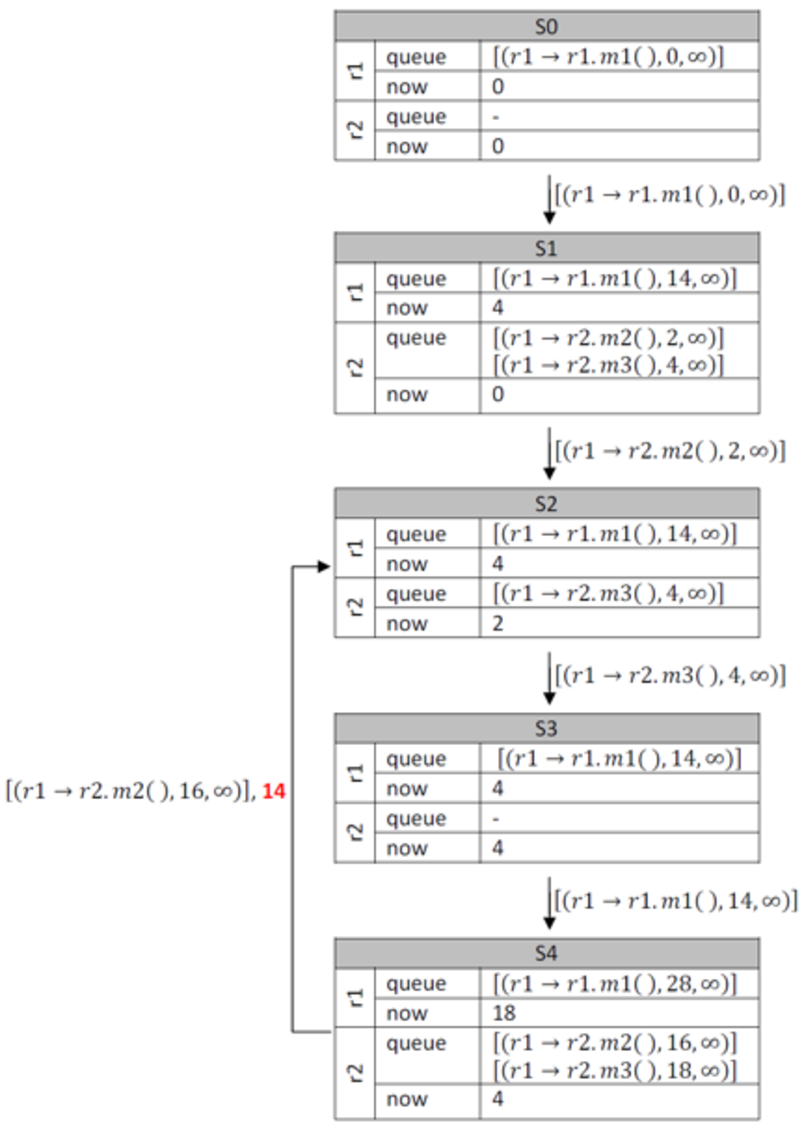
\includegraphics[width=.35\textwidth]{Picture3-BFTTS.pdf}
\caption{ Bounded FTTS for the Timed Rebeca model in Listing \ref{src::FTTS-actor-model}.}
\label{fig::FTTSandTTS}
\end{figure}

\section{Distributed Model Checking} \label{sec::DMC}
In addition to benefiting from the isolation of actors for reducing the size of state spaces, this property can be used for more efficient analysis of huge state spaces. A major limiting factor in applying model checking for the analysis of real-world systems is the huge amount of memory space and time required to store and explore state spaces. Distributed model checking is a technique for analyzing the state space in which it is partitioned into slices and each slice is assigned to a computational node to be analyzed. Efficiency of this technique depends on the number of required communications among the computational nodes which is affected by the distribution policy of states among the nodes \cite{DBLP:journals/entcs/OrzanPE05}. 
%
%Another, more fine-grained, representative of communication cost 
To reduce the number of required communications, split transitions have to be avoided; a split transition is a transition between two states where the hosts of the source and destination states are located at different nodes. In \cite{DBLP:journals/eceasst/KhamespanahSMSR15} we show how the actor model can be used to reduce the number of split transitions. We introduce a new state distribution policy based on the so-called \textit{Call Dependency Graph (CDG)} of actor models. A CDG represents the abstract causality relation among messages of actors. Our abstraction is akin to the Clinger's event diagram \cite{clinger} that shows the causality among events which are sent by actors of the system in their life times. Note that sent messages in CDG are interpreted as events in the Clinger's event diagram.

The most primitive and widely used distribution policy is random state distribution \cite{DBLP:journals/entcs/GaravelMS13}. Random state distribution policy distributes states among nodes based on their hash values. Random distribution policy guarantees load balancing. However, it is not an effective technique as cycles in the state space are scattered over many different nodes. Note that detecting cycles of state spaces is crucial for model checking against LTL-like properties; so, splitting them among nodes (i.e., reducing locality of cycles) dramatically increases the model checking time consumption. In \cite{DBLP:journals/entcs/OrzanPE05}, another state space distribution policy is suggested to improve the locality of cycles. This policy is based on the static analysis of an abstracted model and detects \emph{may} or \emph{must} transition relations among states \cite{DBLP:conf/lics/LarsenT88}.
\fixme{define may and must in one sentence}
Based on this analysis, if two states have a \emph{must} relation, they should be stored in a same node. We use a similar idea in our state distribution policy using CDG by partitioning causality relations of CDGs to \emph{may} and \emph{must} relations. So, we detect the \emph{must} relations among the states of an actor model considering the cycles of its corresponding CDG and putting them in the same node. Our technique is applicable to other distributed systems where the unit of concurrency can be modeled as isolated autonomous reactive objects and message passing is the only means of communication. 

Clinger's event diagram comprises vertices (called \emph{dots}) for each event, and edges (called \emph{arrows}) that represent the activation relation of two events. Clinger's event diagram is typically drawn using parallel vertical swim-lanes for each actor, where the dots are placed for each event respecting their sequential execution order. Figure~\ref{fig::clinger} represents the Clingers' event diagram of a simple actor model, shown in Listing~\ref{src::actor-model}. 

\begin{lstlisting}[language=rebeca, caption= A simple actor model, label=src::actor-model]
reactiveclass AC1 {
   knownrebecs {AC2 ac2;}
   AC1() {
     self.msg1();
   }
   msgsrv msg1() {
     self.msg2();
     ac2.msg3();
   }
   msgsrv msg2() {
     self.msg1();
     ac2.msg4();
   }
}
reactiveclass AC2 {
   knownrebecs{AC1 ac1;}
   statevars{int sv;}
   AC2() {
     sv = 1;
   }
   msgsrv msg3() {
     ac1.msg1();
   }
   msgsrv msg4() {
     if (sv == 1)
       sv = 4;
     else
       sv = 3;
   }
}
main {
    AC1 ac1(ac2):();
    AC2 ac2(ac1):();
}
\end{lstlisting}

Clinger's event diagrams can be seen as the detailed representations of CDG. As actors are isolated, the only causality relation among events is expressed by sending a message. So, the causality relation of events in a CDG can be extracted from the source codes of actor models using static analysis. This way, we over-approximate the causality relations in CDGs. Figure \ref{fig::cdg} illustrates the CDG which corresponds to the Clinger's event diagram of Figure \ref{fig::clinger}.

\begin{figure}
\centering
%\subfigure[Clinger event diagram of the actor model in Listing \ref{src::actor-model}]{
\begin{subfigure}[b]{0.2\textwidth}
  \centering
  \small{
   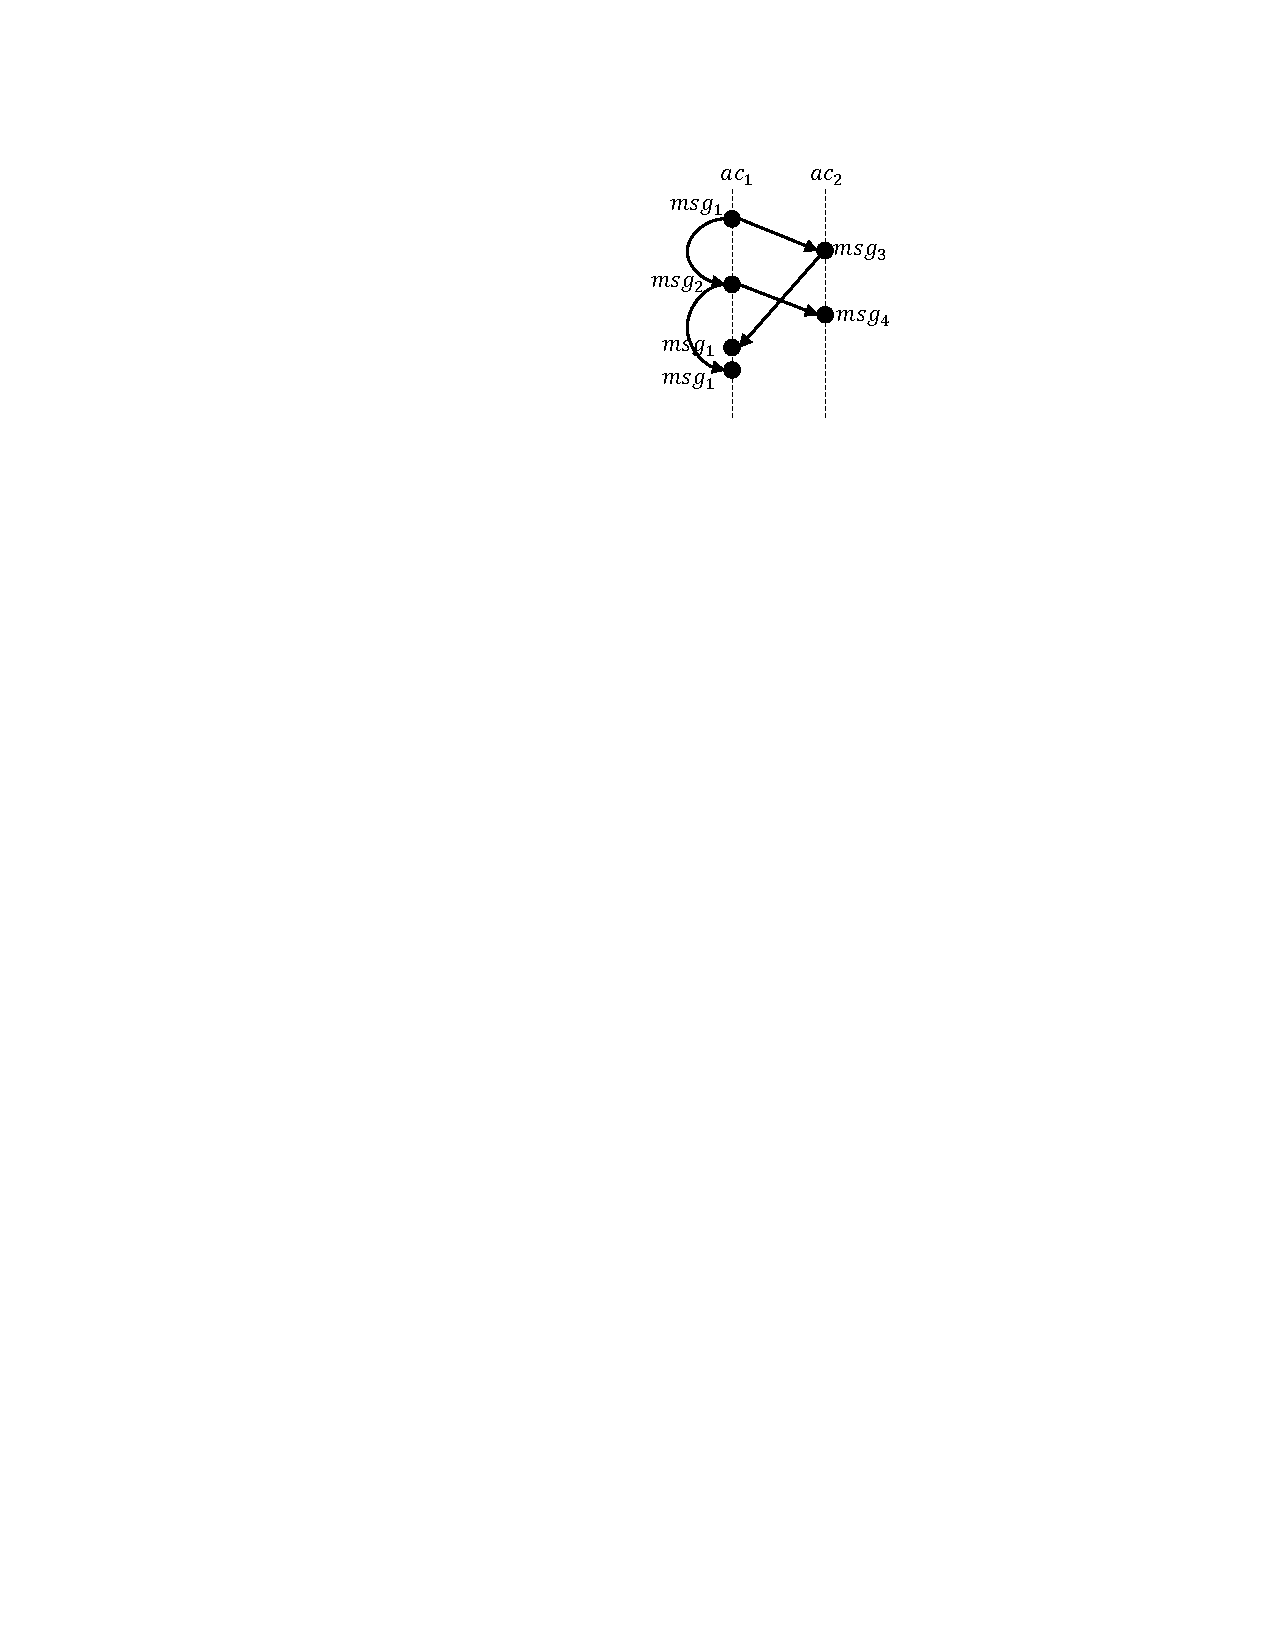
\includegraphics[width=.8\textwidth]{resources/clinger.pdf}
  }
  \caption{Clinger event diagram of the actor model in Listing \ref{src::actor-model}}
  \label{fig::clinger}
%}
\end{subfigure}
\qquad
\begin{subfigure}[b]{0.2\textwidth}
%\subfigure[CDG of the actor model in Listing 1]{

  \centering
  \small{
   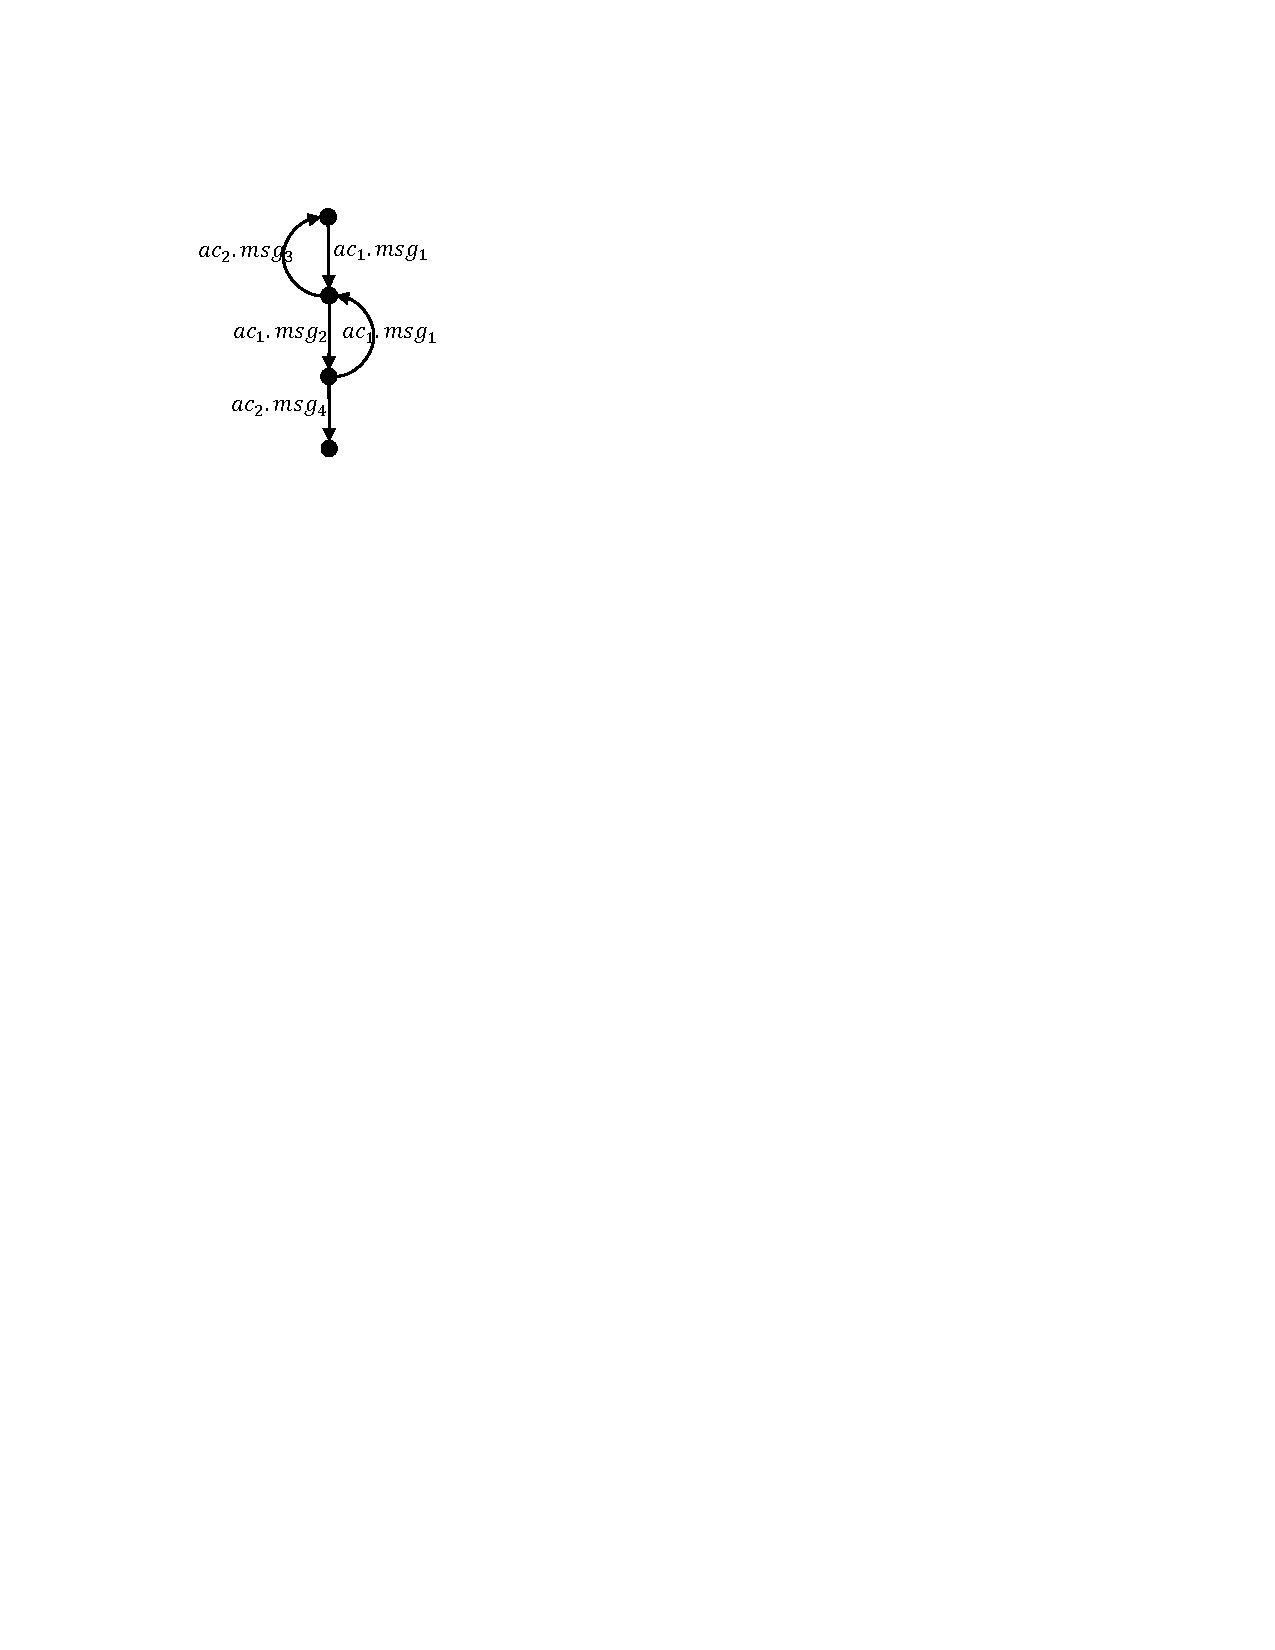
\includegraphics[width=.8\textwidth]{resources/cdg.pdf}
  }
  \caption{CDG of the actor model in Listing \ref{src::actor-model}}
  \label{fig::cdg}
%}
\end{subfigure}
\caption{Clinger event diagram versus CDG of the actor model in Listing \ref{src::actor-model}.}
\label{fig::clinger-cdg}
\end{figure}

We designated the existence of a relation between the cycles in a CDG and the cycles in its corresponding state space in \cite{DBLP:journals/eceasst/KhamespanahSMSR15}. \Fatem{It is not clear that how isolation helps in resolving this issue}. 
As mentioned before, Rebeca actors are completely isolated and the only way of expressing causality among events is the message passing mechanism, explicitly specified in Rebeca models. Experimental evidence supports that this new policy improves cycles locality, and decreases the model checking time and memory consumption in practice.
\section{Verification of Mobile Ad-hoc Protocols}\label{sec::wrebeca} 
Mobile Ad-hoc wireless networks (MANETs) consist of mobile nodes equipped by wireless transceivers by which they communicate. These networks are applicable where no pre-existing infrastructure, such as routers in wired networks or access points in wireless networks 
are available.  
%as their nodes operate in a completely collaborative and distributed manner.
Node $A$ can receive data from  node $B$ if $A$ is located in the communication range of $B$, i.e., $A$ is directly connected to $B$. The union of connectivity/disconnectivity relations among nodes forms the underlying topology.  In such networks, nodes can freely move, so the %connectivity/disconnectivity relations may change, and the 
topology dynamically changes. As all nodes are not directly connected, they rely on each other to communicate indirectly with those not within their range. To this aim, they collaborate ad-hocly to find a valid route from a source to a destination. A route is valid if the corresponding path exists in the topology. Routes are partially maintained in the routing tables of nodes by indicating the next-hop(s) via which an intended destination is accessible. As topology changes, the routes maintained by nodes should be updated to prevent using  invalid routes. % leading to the energy consumption and network degradation. 
During the process of route maintenance, it is possible that by following next-hops, a route visits the same node more than once, and a loop is formed. 
%Being 
\emph{Loop-freedom} is one of the main required properties of MANET routing protocols. Because the topology is changing all the time, finding a scenario that leads to protocol malfunction (for example  formation of a loop in the routing protocol), is very unlikely if we use  simulation-based approaches. So, these approaches are not very helpful in designing such protocols in practice. 
%Due to the enormous number of topology changes, finding a mobility scenario leading to protocol malfunction, e.g., the formation of a loop for routing protocols, is not possible by simulation-based approaches, and so these approaches can not assist in designing such protocols in practice.   


An extension of Rebeca, called wRebeca, is introduced in \cite{FOAC}, and is used to 
model and verify MANET protocols addressing dynamically changing topology. To support modeling such protocols, wRebeca provides \textit{unicast}, \textit{multicast}, and \textit{broadcast} for communication. The wRebeca model of an abstract version of Ad-hoc On Demand Vector (AODV) routing protocol \cite{AODV} is given in Figure \ref{code:aodv}. Each node in the network is represented as an actor while the routing protocol is modeled through the message servers of the actor. The network topology and its mobility 
%are addressed by the state transition system, 
%the third level of abstraction, and 
are not explicitly modeled in the wRebeca code, instead we address them at the level of the state transition system.  In message server ${\it rec\_newpkt}$ (line $10$),
whenever a source node intends to send a data packet to a destination (${\it dip\_}$), first it looks up in its routing table, ${\it rst}[{\it dip\_}]$, to see if it has a valid route to the destination to forward the data packet. Otherwise it starts a route discovery by broadcasting a route request message, ${\it rec\_rreq}$, at line $16$. Nodes upon processing a request message, forward the request (line $38$) if they do not have any route to the destination until the request reaches to the destination (line $24$). The destination replies by unicasting a reply message, ${\it rec\_rrep}$, in response (line $26$) to the sender of the request (${\it oip\_}$), called origin. As links may not be bidirectional, the origin may not be directly connected to the destination, so the destination unicasts to the next-hop towards the origin (${\it nhop}[{\it oip\_}]$). The modeler can specify what should be done in case the unicast message is delivered
successfully ($\it succ$ in line $28$) %if the receiver node is in the wireless range,
or the delivery fails ($\it unsucc$ in line $31$). %if the receiver node is not in the wireless range. 
The reply message is resent by the middle nodes (line $50$) until it arrives to the source node (line $47$).
%\Marjan{you said the topology is at the level of the transition system, then how this succ and unsucc are handled?}\Fatem{The effect of communication operators are handled regarding the topology at the semantics. The modeler states what should executed if a unicast is succ/unsucc }


\begin{figure*}
	\begin{center}
		%	\begin{lstlisting}[language=rebeca,multicols=2]
		\input{AODV-min.txt}
		%	\end{lstlisting}
	\end{center}
	\caption{The AODV protocol specified by wRebeca \label{code:aodv}\cite{FOAC}}
\end{figure*} 

To reason about MANET protocols by  model checking technique, the state transition systems of their models have to be generated. In wRebeca tool, the global states (denoted as $(S,\gamma)$) are defined by the local states of rebecs and the underlying topology.
%
%the global states are defined by the local states of rebecs and the underlying topology, denoted by $(S,\gamma)$. 
The state-space generator produces two types of transitions; transitions for atomic handling of messages in the actor queues, and transitions for random modification of the underlying topology to address mobility. A resulting state space %has been 
is shown partially in Figure \ref{Fig::stbefore}. The message handling transitions are represented by $a/b$-transitions while random modification of the topology is shown by $\tau$-transitions. %For generating the first type, the effect of communication statements like broadcast is computed with respect to the topology.
For generating the first type of transition, the effect of communication statements, like broadcast, on the topology is considered.
When an actor broadcasts, only those that are directly connected to the sending actor will receive the message. We remark that the underlying topology is not changed by the first type of transitions, for example note the following transitions in Figure \ref{Fig::stbefore}:  $(S_0,\gamma_1)\overto{a}(S_1,\gamma_1)$  and $(S_0,\gamma_1)\overto{b}(S_2,\gamma_1)$. For a network of $n$ nodes, there are $2\times \begin{pmatrix}
n \\
2 \\
\end{pmatrix}$ possible uni-directional links among the nodes, and as each link can be up/down, there are $2^{(n^2-n)}$ possible topologies. So, for each global state, $2^{(n^2-n)}$ transitions are generated to randomly change the topology, and the state space grows exponentially, resulting state-space explosion. It is notable that the local states of rebecs are not changed by $\tau$-transitions like $(S_1,\gamma_1)\overto{\tau}(S_1,\gamma_2)$ and $(S_2,\gamma_1)\overto{\tau}(S_2,\gamma_3)$.

\begin{figure}[h]
\begin{subfigure}[b]{0.32\textwidth}
%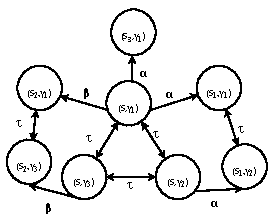
\includegraphics[width=\textwidth]{resources/st-before.pdf}
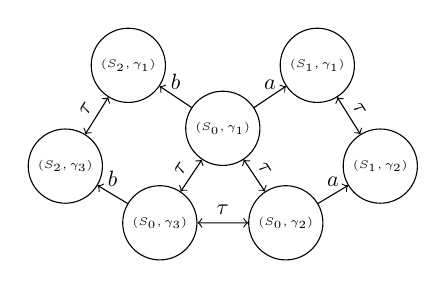
\begin{tikzpicture}[scale=.8, transform shape]		
\node[circle,draw] (n1) at (0,0) {\tiny$(S_0,\gamma_1)$};
\node[circle,draw] (n2) at (1,-1.5) {\tiny$(S_0,\gamma_2)$};
\node[circle,draw] (n3) at (-1,-1.5) {\tiny$(S_0,\gamma_3)$};
\node[circle,draw] (n4) at (1.5,1) {\tiny$(S_1,\gamma_1)$};
\node[circle,draw] (n5) at (2.5,-0.6) {\tiny$(S_1,\gamma_2)$};
\node[circle,draw] (n6) at (-1.5,1) {\tiny$(S_2,\gamma_1)$};
\node[circle,draw] (n7) at (-2.5,-0.6) {\tiny$(S_2,\gamma_3)$};
%\node[circle,draw] (n8) at (0,1.6) {\tiny$(S_3,\gamma_1)$};
\draw[<->]  (n1) edge node[above,sloped]{$\tau$} (n2);
\draw[<->]  (n1) edge node[above,sloped]{$\tau$} (n3);
\draw[<->]  (n2) edge node[above,sloped]{$\tau$} (n3);
\draw[<->]  (n5) edge node[above,sloped]{$\tau$} (n4);
\draw[<->]  (n6) edge node[above,sloped]{$\tau$} (n7);
%\draw[->]  (n1) edge node[right]{$a$} (n8);
\draw[->]  (n1) edge node[above]{$a$} (n4);
\draw[->]  (n1) edge node[above]{$b$} (n6);
\draw[->]  (n2) edge node[above]{$a$} (n5);
\draw[->]  (n3) edge node[above]{$b$} (n7);
\end{tikzpicture}
\caption{Before reduction}\label{Fig::stbefore}	
\end{subfigure}
\begin{subfigure}[b]{0.14\textwidth}
%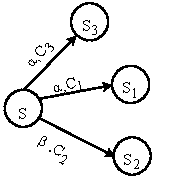
\includegraphics[width=\textwidth]{resources/st-after.pdf}
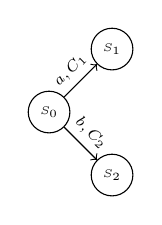
\begin{tikzpicture}[scale=.8, transform shape]			
\node[circle,draw] (n1) at (0,0) {\tiny$S_0$};
\node[circle,draw] (n2) at (1,1) {\tiny$S_1$};
\node[circle,draw] (n3) at (1,-1) {\tiny$S_2$};
%\node[circle,draw] (n4) at (1.5,0) {\tiny$S_3$};
\draw[->]  (n1) edge node[above,sloped]{\scriptsize$a,C_1$} (n2);
\draw[->]  (n1) edge node[above,sloped]{\scriptsize $b,C_2$} (n3);
%\draw[->]  (n1) edge node[above]{\scriptsize$a,C_3$} (n4);
\end{tikzpicture}
\caption{After reduction}\label{Fig::stafter}	
\end{subfigure}
\caption{A simple state space before and after applying the reduction. The network constraint $C_1$ expresses the common links of the topologies $\gamma_{1}$ and $\gamma_2$ while $C_2$ represents the common links of $\gamma_1$ and $\gamma_3$. %, and $C_3$ represents the links of $\gamma_1$.
}\label{Fig::reductionidea}	
\end{figure}

To tackle state-space explosion, we propose a symmetric reduction technique that eliminates the topology from the global states and combines those states that are only different in their topologies.  So the states $(S_0,\gamma_1)$, $(S_0,\gamma_2)$, and $(S_0,\gamma_3)$ of Figure \ref{Fig::stbefore} are aggregated to $S_0$ as demonstrated in Figure \ref{Fig::stafter}. As a consequence, transitions modifying the topology are removed (as they become self-loop $\tau$-transitions). 
A state transition like $S_0\overto{a} S_1$ is possible in Figure \ref{Fig::stafter} after the reduction, as we have $(S_0,\gamma_1)\overto{a}(S_1,\gamma_1)$ and $(S_0,\gamma_2)\overto{a}(S_1,\gamma_2)$ in Figure \ref{Fig::stbefore} before the reduction. In other words, when the local states of rebecs is $S_0$ and the underlying topology is either $\gamma_1$ or $\gamma_2$, handling the same message, represented by $a$, leads to the same next local states, i.e., $S_1$.  As message handlers are executed with regard to the topology, the connectivity/disconnectivity of those links that are common in both topologies make the effect of handling the message to be the same. The connectivity/disconnectivity relations of these links, called \emph{network constraint}~\cite{FatemehFI10,FatemehFI19},  are added to the labels on the transitions. For example, the links common in both $\gamma_{1}$ and $\gamma_{2}$ that result in the same next local states, i.e., $S_1$ in Figure \ref{Fig::stbefore}, are added by the network constraint $C_1$ to the label of the transition $S_0\overto{a,C_1}S_1$ in Figure \ref{Fig::stafter}. %For instance, the network constraint ${\it and}({\it con}(n_1,n_2),!{\it con}(n_3,n_4))$ expresses that the actor  $n_1$ is connected to $n_2$ while $n_3$ is disconnected from $n_4$. 
To enforce a set of stable connectivity/disconnectivity relations among the actors, we specify them by a network constraint at the \emph{constraints} block of the model. For instance, the network constraint given in line $68$ of Figure \ref{code:aodv} enforces $n_3$ to be always connected to $n_4$, expressed by ${\it con}(n_3,n_4)$.  
%Our reduction technique is indeed a form of symmetric reduction technique \cite{clarke1998symmetry}. 
As this reduction technique is applied at the transition system level, it can be also applied if the actors were not isolated. However, the non-preemptive execution of event handlers at the model level makes this reduction at the state-space level more effective for the analysis of real-world protocols like AODV. 


\fixme{Here you are talking only about the "atomic execution of methods", right? that we cannot really call isolation ... we should talk about atomic execution of methods and then maybe say why we can do it without loss of generality, that is because of isolation.}
\fixme{I will add the text related to isolation and atomic execution of methods in Section 2, then here you can talk about atomic execution of methods. But we loose genrality if we have some kind of cyclic calling (or two calls from the same sender to the same receiver), I need to ask you if in your application such scenarios are possible or not - we are losing possible interleavings in these scenarios.}
In following we discuss the amount of reductions achieved by combination of the isolation at the model
level and topology elimination at the level of the transition system. The topology-elimination reduction technique eliminates the topology $\gamma$ from the global state $(S,\gamma)$ and generates the next local actor states for handling messages
considering all possible connectivity/disconnectivity of the handling actor to other actors. For a network of $n$ nodes, each node has $2^{n-1}$ possible connectivity/disconnectivity relations with others. So, the topology-elimination reduction technique reduces the number of states from $\mathbb{S}\times 2^{(n^2-n)}$ to $\mathbb{S}\times2^{n-1}$, where $\mathbb{S}$ is the total number of possible local states of actors. If $\mathbb{S}$ be a large number, the reduction achieved by topology-elimination is not sufficient enough for tackling state-space explosion, as we experienced in the algebraic framework of \cite{FORM}. If message handlers were preemptive, $\mathbb{S}$ would be indeed huge because of enormous possible interleaving of message handlers. Restricting to isolated actors, minimizes $\mathbb{S}$ substantially. 
%
%
%Assume a snapshot of a model where we have $k$ actors that each has at least one event in its queue to handle, and the corresponding event handlers of events have $i_1$, $\ldots$, $i_k$ statements in the model. 
%\Fatem{why you have k actors, and also k statements?}
%When actors are not isolated, the local states of actors are defined by triple elements in the micro-step semantics: state variable valuation, queue contents, and the pointer to the statements to be executed (PC). For handling these $k$ events, $m\times 2^{(n^2-n)}$ global states are generated at the micro-step semantic level, where $m$ is the number of possible interleaving of event handler's statements (hence, the number of possible local states). The topology-elimination reduction technique reduces the number of states from $m\times 2^{(n^2-n)}$ to $m\times2^{n-1}$. If $m$ be a large number, the reduction achieved by topology-elimination is not sufficient enough for tackling state-space explosion, as we experienced in the algebraic framework of \cite{FORM}. Restricting to isolated actors, minimizes $m$ substantially.
%
%\fixme{maybe we remove computing of m, remove the following paragraph?}
%We compute $m$ to show that it is indeed large. As there are $i_1+\ldots+i_k$ slots for the statements, we choose $i_1$ in which to place the first event handler statements, $i_2$ of the remaining slots in which to place the second event handler instructions, and so on. This gives the result  ${\small m=\begin{pmatrix}
%	%\displaystyle\sum_{j=1}^{k} i_j \\
%	i_1+\ldots+i_k\\
%	i_1 \\
%	\end{pmatrix}\times
%	\begin{pmatrix}
%	%\displaystyle\sum_{j=2}^{k} i_j \\
%	i_2+\ldots+i_k\\
%	i_2 \\
%	\end{pmatrix}\times	\ldots\times
%	\begin{pmatrix}
%	%\displaystyle\sum_{j=k}^{k} i_j \\
%	i_k\\
%	i_k \\
%	\end{pmatrix}}$ which equals to ${\small %\frac
%{(\sum_{j=1}^{k} i_j)!}/{\prod_{j=1}^{k}(i_j!)}.}$ 
%Restricting to isolated actors, minimizes $m$ substantially to $k!$. The combination of isolation at the model and topology-elimination reduction approach at the semantics shrinks the state space substantially for real-world protocols and hence, makes the model checking technique possible as shown in Table \ref{Tab:aodv-redu}. 
%
Table \ref{Tab:aodv-redu} illustrates the amount of reduction achieved by applying topology-elimination reduction on isolated actors. When the number of nodes increases from $4$ to $5$ for AODV while the specified network constraint at the model results only $16$ possible topologies, the state space cannot be generated due to the memory limitation on a computer with $8${GB} {RAM}.  We proved that the reduced state space is branching bisimilar to the
original one, and consequently a set of properties such as {ACTL-X} are preserved \cite{FOAC}. The network constraints on transition are used during model checking \cite{FORM,CSI2018} to verify the topology-sensitive properties. 

\begin{table*}
	%   \renewcommand{\arraystretch}{1.5}
	\centering
	\caption{Comparing the size of state spaces with/without applying reduction \cite{FOAC}}
	\begin{tabular*}{0.75\textwidth}{@{\extracolsep{\fill }} |   c  c  r  r  r  r  |   }
		\hline
		No. of & No. of valid & No. of states    &  No. of transitions     & No. of states & No. of transitions
		\\
		nodes & topologies & before reduction  &  before reduction   & after reduction &  after reduction
		\\
		\hline	     
		4 & 4 & 3,007 & 16,380 & 763  & 1,969 \\
		4  & 8 & 12,327 & 113,480 & 1,554  & 3,804 \\
		4  & 16 & 35,695 & 610,816 & 2,245 & 5,549 \\    
		4  & 32 & 93,679 & 3,097,792 & 2,942 & 7,596 \\  
		4    & 64  & 258,447  & 16,797,536 & 4,053 & 10,629 \\
		5 & 16 & $>$655,441 & $>$11,276,879 & 165,959 &  598,342 \\
		\hline
	\end{tabular*}
	\label{Tab:aodv-redu}
\end{table*}


\section{Verification of Hybrid Reactive Systems}\label{sec::HRebeca}
Embedded systems consist of microprocessors which control physical behavior. In such \emph{hybrid} systems, physical and cyber behaviors, characterized as continuous and discrete respectively, affect each other; the physical components may trigger the cyber components which change (by (de)activating) physical components in response. The new generation of embedded systems, cyber-physical systems (CPSs) composed of microprocessors controlling other software/physical systems via networks. For instance, in automotive systems, there are components like sensors, actuators, and controllers that communicate asynchronously with each other through a CAN network. The computational model of Rebeca provides a suitable level of abstraction to faithfully model such distributed asynchronously communicating systems in an intuitive way.

Timed Rebeca was extended by Hybrid Rebeca [] with physical behavior to support hybrid systems. Such an extension allows non-determinism inherent in concurrent and distributed systems, e. g., in the case of simultaneous arrival of messages (and no explicit priority-based policy to choose one over the other) to model check the possible implementations of systems. In Hybrid Rebeca, physical behaviors are encapsulated in so-called physical actors. Each physical actor, in addition to message handlers, is defined by a set of modes. Each mode defines the continuous behavior of the actor. A physical actor (which is instantiated from a physical class) must always have one active mode. By changing the active mode of a physical actor, it's possible to change the continuous behavior of the actor. The active mode can be changed upon receiving a message from either a software actor (controller) or a physical actor. The semantics of Hybrid Rebeca is defined as a hybrid automaton, for which many verification algorithms and tools are available. 

We have shown that by using Hybrid Rebeca, the cost of improving and modifying models is vastly reduced compared to modeling in hybrid automata [] as the computational model of Hybrid Rebeca encapsulates many complexities. These complexities subsume high-level concepts like message passing and message buffering. Furthermore, modeling these complexities directly in hybrid automata can hugely decrease the analyzability of the models. Concluding that the abstraction resulted from choosing actors as the basic units of computation, offers more friendliness towards cyber-physical systems compared to the low-level languages like hybrid automata.
	
	
	
	\section*{Acknowledgment}
	\section*{References}
	
	\bibliography{ref}
	\bibliographystyle{plain}
	
	%\begin{thebibliography}{00}
	
	%\end{thebibliography}
	
\end{document}
